
%----------------------------------------------------------------------------------------
%	Settings and packages
%----------------------------------------------------------------------------------------

\documentclass[10pt]{article}

\usepackage{colortbl}
\usepackage{multirow}
\usepackage[table]{xcolor}
\usepackage{ctable}
\usepackage{float}
\usepackage{adjustbox}
\usepackage[landscape,margin=0.25in,legalpaper]{geometry}

\newcommand{\mcn}[2]{\multicolumn{#1}{l}{#2}}	
\newcommand{\mccn}[2]{\multicolumn{#1}{c}{#2}}
\newcommand{\mcl}[1]{\multicolumn{2}{l}{#1}}
\newcommand{\mclg}[1]{\multicolumn{2}{l}{\gr #1}}
\newcommand{\mcc}[1]{\multicolumn{2}{c}{#1}}
\newcommand{\mccg}[1]{\multicolumn{2}{c}{\gr #1}}
\newcommand{\mr}[1]{\multirow{-2}{*}{#1}}
\definecolor{Gray}{gray}{0.90}
\newcommand{\gr}{\cellcolor{Gray}}

\newcommand{\thickline}{\specialrule{.1em}{.05em}{.05em}}

\setlength\parindent{0pt}

% column colours
\newcolumntype{g}{>{\columncolor{Gray}}l}
\newcolumntype{w}{>{\columncolor{white}}l}

%----------------------------------------------------------------------------------------
%	Table
%----------------------------------------------------------------------------------------

\begin{document}

\thispagestyle{empty}
{\bf 2018 Deepwell Cup}
\begin{table}[h!]
  \centering
  \adjustbox{max width=\textwidth}{
    \begin{tabular}{l g g w w g g w w g g w w g g w w g g w w g g w w g g}
        \rowcolor{black}\mcn{27}{\color{white}\bf Round 4: Stanley Cup Finals} \\
        \rowcolor{white}\\
        & \mccg{Andre D} & \mcc{Andres M} & \mccg{Andrew N} & \mcc{Anthony C} & \mccg{Brian M} & \mcc{David D} & \mccg{Jackson L} & \mcc{Josh H} & \mccg{Kollin H} & \mcc{Kyle L} & \mccg{Michael D} & \mcc{Romulus} & \mccg{Ron K}  \\\thickline
        \\\hline
          Vegas Golden Knights&&&&&&&&&&&&&&&&&&&&&&&&&&\\
          Washington Capitals & \mr{VGK} & \mr{7} & \mr{WSH} & \mr{6} & \mr{WSH} & \mr{5} & \mr{WSH} & \mr{5} & \mr{VGK} & \mr{6} & \mr{VGK} & \mr{5} & \mr{VGK} & \mr{4} & \mr{VGK} & \mr{5} & \mr{VGK} & \mr{5} & \mr{WSH} & \mr{6} & \mr{WSH} & \mr{6} & \mr{VGK} & \mr{7} & \mr{WSH} & \mr{7}\\\hline
          \rowcolor{white}\\
        \rowcolor{black} \mcn{27}{\color{white}\bf Conference Champions} \\
          Eastern & \mclg{WSH} & \mcl{PIT} & \mclg{TOR} & \mcl{TBL} & \mclg{TBL} & \mcl{CBJ} & \mclg{WSH} & \mcl{TBL} & \mclg{BOS} & \mcl{TBL} & \mclg{WSH} & \mcl{NJD} & \mclg{TOR}\\
          Western & \mclg{VGK} & \mcl{NSH} & \mclg{MIN} & \mcl{NSH} & \mclg{WPG} & \mcl{WPG} & \mclg{SJS} & \mcl{WPG} & \mclg{NSH} & \mcl{WPG} & \mclg{NSH} & \mcl{WPG} & \mclg{WPG}\\
          Stanley Cup & \mclg{VGK} & \mcl{PIT} & \mclg{MIN} & \mcl{NSH} & \mclg{TBL} & \mcl{WPG} & \mclg{SJS} & \mcl{TBL} & \mclg{NSH} & \mcl{WPG} & \mclg{TBL} & \mcl{NJD} & \mclg{NSH}
    \end{tabular}
  }
\end{table}

{\bf Points}\\
\begin{minipage}[t]{10cm}
    \vspace{0pt}
    \begin{tabular}{l l}
        Let $C$ be the correct number of games\\
        Let $P$ be the predicted number of games\\
        If correct team chosen:	   & $9 - \left|{C - P}\right|$\\
        if incorrect team chosen:  & $C + P - 8$\\
        Stanley Cup champion:	& 3\\
        Stanley Cup finalist:	& 3\\
    \end{tabular}

    \vspace{0.5cm}
    {\bf Number of picks:}\\
    \begin{tabular}{lc }
        VGK & 7 \\
        WSH & 6 \\
    \end{tabular}
\end{minipage}
%
\begin{minipage}[t]{4cm}
    \vspace{0pt}
    \qquad Correct team Points\\
    \begin{tabular}{c l | c c c c }
        \mccn{2}{} & \mccn{4}{Predicted}\\
        & & 4 & 5 & 6 & 7\\\cline{2-6}
        \parbox[t]{2mm}{\multirow{4}{*}{\rotatebox[origin=c]{90}{Correct}}} & 4 & 9 & 8 & 7 & 6\\
        & 5 & 8 & 9 & 8 & 7\\
        & 6 & 7 & 8 & 9 & 8\\
        & 7 & 6 & 7 & 8 & 9
    \end{tabular}
\end{minipage}
%
\begin{minipage}[t]{4cm}
    \vspace{0pt}
    \qquad Incorrect team Points\\
    \begin{tabular}{c l | c c c c }
        \mccn{2}{} & \mccn{4}{Predicted}\\
        & & 4 & 5 & 6 & 7\\\cline{2-6}
        \parbox[t]{2mm}{\multirow{4}{*}{\rotatebox[origin=c]{90}{Correct}}} & 4 & 0 & 1 & 2 & 3\\
        & 5 & 1 & 2 & 3 & 4\\
        & 6 & 2 & 3 & 4 & 5\\
        & 7 & 3 & 4 & 5 & 6
    \end{tabular}
\end{minipage}
%
\begin{minipage}[t]{13cm}
    \vspace{0pt}
    \begin{figure}[H]
        \vspace{-1cm}
        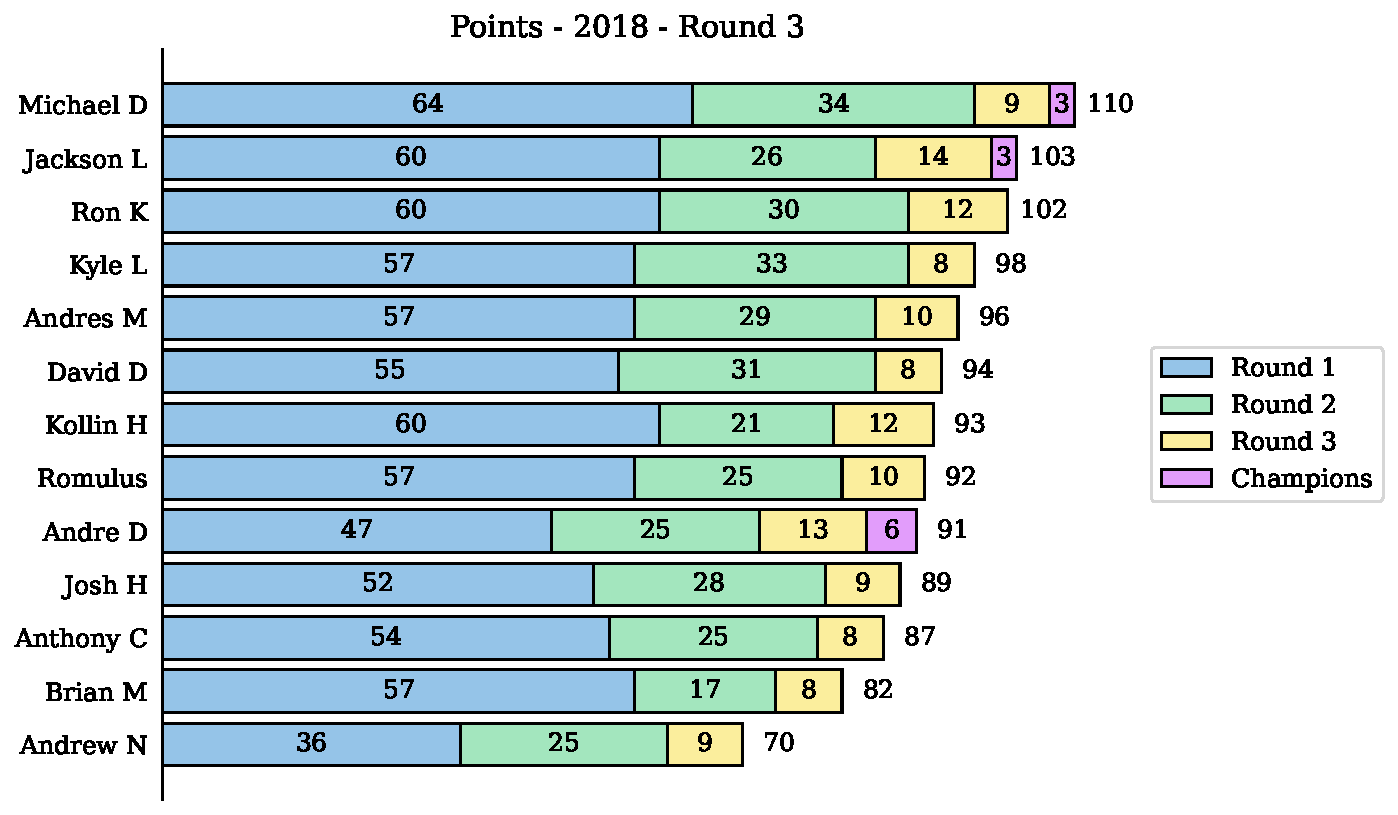
\includegraphics[width=12cm,height=8cm,keepaspectratio]{../../figures/2018/Points-2018-Round3.pdf}
    \end{figure}
\end{minipage}

\end{document}